% Options for packages loaded elsewhere
\PassOptionsToPackage{unicode}{hyperref}
\PassOptionsToPackage{hyphens}{url}
\documentclass[
  11pt,
]{article}
\usepackage{xcolor}
\usepackage[left=3cm,right=3cm,top=2.5cm,bottom=2.5cm]{geometry}
\usepackage{amsmath,amssymb}
\setcounter{secnumdepth}{5}
\usepackage{iftex}
\ifPDFTeX
  \usepackage[T1]{fontenc}
  \usepackage[utf8]{inputenc}
  \usepackage{textcomp} % provide euro and other symbols
\else % if luatex or xetex
  \usepackage{unicode-math} % this also loads fontspec
  \defaultfontfeatures{Scale=MatchLowercase}
  \defaultfontfeatures[\rmfamily]{Ligatures=TeX,Scale=1}
\fi
\usepackage{lmodern}
\ifPDFTeX\else
  % xetex/luatex font selection
\fi
% Use upquote if available, for straight quotes in verbatim environments
\IfFileExists{upquote.sty}{\usepackage{upquote}}{}
\IfFileExists{microtype.sty}{% use microtype if available
  \usepackage[]{microtype}
  \UseMicrotypeSet[protrusion]{basicmath} % disable protrusion for tt fonts
}{}
\usepackage{setspace}
\makeatletter
\@ifundefined{KOMAClassName}{% if non-KOMA class
  \IfFileExists{parskip.sty}{%
    \usepackage{parskip}
  }{% else
    \setlength{\parindent}{0pt}
    \setlength{\parskip}{6pt plus 2pt minus 1pt}}
}{% if KOMA class
  \KOMAoptions{parskip=half}}
\makeatother
\usepackage{longtable,booktabs,array}
\usepackage{caption}
\captionsetup[table]{skip=6pt}
\newcounter{none} % for unnumbered tables
\usepackage{calc} % for calculating minipage widths
% Correct order of tables after \paragraph or \subparagraph
\usepackage{etoolbox}
\makeatletter
\patchcmd\longtable{\par}{\if@noskipsec\mbox{}\fi\par}{}{}
\makeatother
% Allow footnotes in longtable head/foot
\IfFileExists{footnotehyper.sty}{\usepackage{footnotehyper}}{\usepackage{footnote}}
\makesavenoteenv{longtable}
\usepackage{graphicx}
\makeatletter
\newsavebox\pandoc@box
\newcommand*\pandocbounded[1]{% scales image to fit in text height/width
  \sbox\pandoc@box{#1}%
  \Gscale@div\@tempa{\textheight}{\dimexpr\ht\pandoc@box+\dp\pandoc@box\relax}%
  \Gscale@div\@tempb{\linewidth}{\wd\pandoc@box}%
  \ifdim\@tempb\p@<\@tempa\p@\let\@tempa\@tempb\fi% select the smaller of both
  \ifdim\@tempa\p@<\p@\scalebox{\@tempa}{\usebox\pandoc@box}%
  \else\usebox{\pandoc@box}%
  \fi%
}
% Set default figure placement to htbp
\def\fps@figure{htbp}
\makeatother
% definitions for citeproc citations
\NewDocumentCommand\citeproctext{}{}
\NewDocumentCommand\citeproc{mm}{%
  \begingroup\def\citeproctext{#2}\cite{#1}\endgroup}
\makeatletter
 % allow citations to break across lines
 \let\@cite@ofmt\@firstofone
 % avoid brackets around text for \cite:
 \def\@biblabel#1{}
 \def\@cite#1#2{{#1\if@tempswa , #2\fi}}
\makeatother
\newlength{\cslhangindent}
\setlength{\cslhangindent}{1.5em}
\newlength{\csllabelwidth}
\setlength{\csllabelwidth}{3em}
\newenvironment{CSLReferences}[2] % #1 hanging-indent, #2 entry-spacing
 {\begin{list}{}{%
  \setlength{\itemindent}{0pt}
  \setlength{\leftmargin}{0pt}
  \setlength{\parsep}{0pt}
  % turn on hanging indent if param 1 is 1
  \ifodd #1
   \setlength{\leftmargin}{\cslhangindent}
   \setlength{\itemindent}{-1\cslhangindent}
  \fi
  % set entry spacing
  \setlength{\itemsep}{#2\baselineskip}}}
 {\end{list}}
\usepackage{calc}
\newcommand{\CSLBlock}[1]{\hfill\break\parbox[t]{\linewidth}{\strut\ignorespaces#1\strut}}
\newcommand{\CSLLeftMargin}[1]{\parbox[t]{\csllabelwidth}{\strut#1\strut}}
\newcommand{\CSLRightInline}[1]{\parbox[t]{\linewidth - \csllabelwidth}{\strut#1\strut}}
\newcommand{\CSLIndent}[1]{\hspace{\cslhangindent}#1}
\setlength{\emergencystretch}{3em} % prevent overfull lines
\providecommand{\tightlist}{%
  \setlength{\itemsep}{0pt}\setlength{\parskip}{0pt}}
%% tools/stamp.tex
%% Provenance footer for PDFs rendered from this project.
%% Vendored by zzcollab; this file is not project-specific. The
%% footer prints the source document and the time of rendering.
%% The git version is defined here too, and so is available to a
%% project that wants it on the page, but it is left off the
%% default footer: it already names the staged copy in share/ and
%% appears in its manifest row. All values are supplied at render
%% time by tools/stamp-render.R, which writes a small generated
%% file that redefines the macros below. The \providecommand
%% defaults keep a bare LaTeX compile working when the document is
%% built without the wrapper.
\usepackage{fancyhdr}
\usepackage{xcolor}
\providecommand{\stampsource}{\detokenize{(source not recorded)}}
\providecommand{\stamptime}{(time not recorded)}
\providecommand{\stampversion}{\detokenize{(version not recorded)}}
\setlength{\footskip}{40pt}
\newcommand{\stampfootcontent}{%
  \footnotesize\color{gray}%
  \parbox[b]{\textwidth}{%
    \stamptime\hfill\thepage\\[2pt]%
    \ttfamily\raggedright\stampsource}}
\pagestyle{fancy}
\fancyhf{}
\fancyfoot[C]{\stampfootcontent}
\renewcommand{\headrulewidth}{0pt}
\renewcommand{\footrulewidth}{0.4pt}
%% The title page uses the `plain` page style; redefine it so the
%% stamp appears there too.
\fancypagestyle{plain}{%
  \fancyhf{}%
  \fancyfoot[C]{\stampfootcontent}%
  \renewcommand{\headrulewidth}{0pt}%
  \renewcommand{\footrulewidth}{0.4pt}}
\renewcommand{\stampsource}{\textasciitilde{}/\allowbreak{}prj/\allowbreak{}res/\allowbreak{}09-summary-stats-efficacy/\allowbreak{}summarystats/\allowbreak{}analysis/\allowbreak{}report/\allowbreak{}report.Rmd}
\renewcommand{\stamptime}{2026-08-20 20:11 PDT}
\renewcommand{\stampversion}{\detokenize{7b468d2-wip}}
\usepackage{amsmath}
\usepackage{amssymb}
\usepackage{booktabs}
\usepackage{longtable}
\usepackage{float}
\usepackage[mathlines]{lineno}
\linenumbers
\usepackage{booktabs}
\usepackage{longtable}
\usepackage{array}
\usepackage{multirow}
\usepackage{wrapfig}
\usepackage{float}
\usepackage{colortbl}
\usepackage{pdflscape}
\usepackage{tabu}
\usepackage{threeparttable}
\usepackage{threeparttablex}
\usepackage[normalem]{ulem}
\usepackage{makecell}
\usepackage{xcolor}
\usepackage{bookmark}
\IfFileExists{xurl.sty}{\usepackage{xurl}}{} % add URL line breaks if available
\urlstyle{same}
% fallback for those not using the hyperref driver hyperxmp:
\makeatletter
\@ifundefined{xmpquote}{\newcommand{\xmpquote}[1]{#1}}{}
\makeatother
\hypersetup{
  pdftitle={Summary statistics for treatment efficacy estimation in clinical trials: when simplicity rivals complexity},
  pdfauthor={Ronald G. Thomas, Ph.D.},
  hidelinks,
  pdfcreator={LaTeX via pandoc}}

\title{Summary statistics for treatment efficacy estimation in clinical trials: when simplicity rivals complexity}
\author{Ronald G. Thomas, Ph.D.\thanks{Wertheim School of Public Health, UCSD; ORCID: 0000-0003-1686-4965}}
\date{August 20, 2026}

\begin{document}
\maketitle

{
\setcounter{tocdepth}{2}
\tableofcontents
}
\setstretch{1.1}
\begin{abstract}
Mixed-model repeated measures (MMRM) is the default primary
analysis for longitudinal continuous endpoints in clinical
trials, but the two-stage summary-measures approach (per-subject
slope or change score, followed by ANCOVA) remains attractive
where covariance misspecification, degrees-of-freedom
controversy, and interpretability are practical concerns. We
synthesize three decades of summary-measures literature and
report a Monte Carlo simulation, under a random-intercept-and-
slope generating model, comparing slope-summary ANCOVA,
change-score ANCOVA, and MMRM on bias, coverage, power, and
Type I error, each scored against its own estimand and each
reported with Morris-Table-6 Monte Carlo standard errors. We
argue that the most defensible framing for summary statistics is
not a claim of general superiority over MMRM, which the
literature (Frison and Pocock; Vossoughi; Ard) has already
established for the linear-divergence setting the current
simulation covers, but a decision-support case grounded in the
ICH E9(R1) estimands framework: the summary-statistic slope
estimand is covariance-model-free and directly interpretable,
while the MMRM visit-specific estimand is conditional on the
working covariance model.
\end{abstract}

\noindent\textbf{Keywords:} summary measures; ANCOVA; MMRM;
longitudinal clinical trials; estimands; Monte Carlo simulation

\section*{Data and code availability}

All simulation code, the manuscript source, and the derived
results object discussed here are version-controlled in the
\texttt{summarystats} repository
(\texttt{analysis/scripts/sim\_study.R},
\texttt{analysis/report/report.Rmd},
\texttt{analysis/data/derived\_data/sim\_09.rds}). No human
subjects data are used; all data are simulated. See the
Reproducibility note at the end of the Results section for the
exact command to regenerate the simulation output.

\section{Introduction}\label{introduction}

Mixed-model repeated measures (MMRM) has become the default
analytic strategy for longitudinal clinical trials with
continuous endpoints. Regulatory agencies and methodological
guidance documents increasingly endorse MMRM as the primary
analysis\textsuperscript{\citeproc{ref-ichE9R12019}{1}}, and the approach has clear theoretical
advantages: it uses all available data under the missing-at-random
(MAR) assumption, accommodates unbalanced designs, and models
complex within-subject correlation structures\textsuperscript{\citeproc{ref-lairdRandomEffectsModels1982}{2}}.

Yet MMRM carries substantial practical burdens. The method
requires specification of a covariance structure, and
misspecification can inflate Type I error or reduce power\textsuperscript{\citeproc{ref-vossoughiSummaryMeasureAnalysis2012}{3}}. Degrees-of-freedom
approximations (Satterthwaite versus Kenward-Roger) remain
unsettled, with different software implementations yielding
discrepant p-values for the same data\textsuperscript{\citeproc{ref-kenwardSmallSampleInference1997}{4},\citeproc{ref-mmrmPackage2024}{5}}.
Convergence failures are common in R packages when fitting
unstructured covariance matrices, particularly with small
samples or many time points. And perhaps most critically, the
MMRM treatment effect estimate at a single visit is not always
intuitive to clinical investigators, who may prefer a single,
interpretable summary of each patient's response trajectory.

An older and simpler tradition, the summary measures
approach, offers a compelling alternative. First articulated
systematically by\textsuperscript{\citeproc{ref-matthewsAnalysisSerialMeasurements1990}{6}},
this two-stage method reduces each subject's repeated
measurements to a single scalar summary (e.g., a slope, area
under the curve, post-treatment mean, or change score) and
then applies standard between-group tests (t-tests, ANCOVA)
to these summaries. The approach requires no covariance
structure specification, yields exact p-values from
well-understood distributions, and produces treatment effect
estimates that are directly interpretable.

We ask whether there exist clinical trial settings in which
summary statistic-based inference is as effective as or superior
to MMRM, and what those settings look like.

\subsection{The summary measures tradition}\label{the-summary-measures-tradition}

The intellectual history of summary measures in clinical trials
spans three decades.\textsuperscript{\citeproc{ref-matthewsAnalysisSerialMeasurements1990}{6}}
introduced the two-stage framework in the BMJ, arguing that the
then-common practice of testing group differences at each time
point was both statistically invalid (due to multiplicity) and
clinically uninformative. They proposed that investigators first
identify a summary that captures the clinically relevant feature
of each patient's trajectory, then analyze these summaries with
simple methods. The approach is statistically valid because the
summaries, being one per subject, are independent across
subjects.

\textsuperscript{\citeproc{ref-frisonRepeatedMeasuresClinical1992}{7}} extended this framework
substantially by demonstrating that when the data can be
summarized by pre-treatment and post-treatment means, analysis
of covariance (ANCOVA) of the post-treatment means adjusted for
the pre-treatment means is the method of choice. They quantified
the superiority of ANCOVA over analysis of post-treatment means
alone and over analysis of change scores, showing that ANCOVA
dominates both in terms of reduced variance and avoidance of
bias. Importantly, they showed that having more than one
pre-treatment measurement provides meaningful gains in
precision, because the pre-treatment mean is a better estimate
of the true baseline than a single observation.

\textsuperscript{\citeproc{ref-frisonLinearlyDivergentTreatment1997}{8}} addressed the case where
treatment effects diverge linearly over time. For this setting,
the natural summary statistic is each subject's regression slope,
and the authors showed that adjusting slopes for baseline values
(or better, for estimated intercepts) yields substantial
efficiency gains. They derived the optimal linear summary
statistic for any repeated measures design with known covariance
structure and known shape of the mean treatment difference,
demonstrating that the summary measures approach can be made
nearly fully efficient.

\textsuperscript{\citeproc{ref-sennRepeatedMeasuresClinical2000}{9}} provided a practical
synthesis, arguing that much repeated measures analysis using
mixed models could be replaced by a summary measures approach
with negligible loss of efficiency. Senn and colleagues described
strategies for baseline adjustment with multiple baselines and
proposed a compromise trend/mean measure (regression through the
origin) useful when both the level and rate of change matter.
They also made the provocative observation that some repeated
measures approaches implicitly violate intention-to-treat
principles, a problem that summary measures avoid.

\subsection{Extensions and refinements}\label{extensions-and-refinements}

\textsuperscript{\citeproc{ref-dawsonStratificationSummaryStatistic1994}{10}} recognized that
summary statistic distributions depend on the pattern of
missingness and proposed stratifying summary statistic tests
by missing data pattern. Simulations showed that stratification
increases power and improves robustness to violations of
missing data assumptions.\textsuperscript{\citeproc{ref-dawsonSampleSizeCalculations1998}{11}}
later provided a unified sample size framework for summary
statistics, covering slopes, post-baseline means, change
scores, and final observations, with modifications for missing
data from staggered entry and random dropouts.

\textsuperscript{\citeproc{ref-weinbergEfficiencyComparisonsRank2001}{12}} examined the efficiency
of rank and permutation tests based on summary statistics under
more complex distributional assumptions, including censored
laboratory markers. Their work demonstrated that the choice of
summary statistic can substantially affect asymptotic relative
efficiency, particularly when the repeated measures exhibit
nonlinear growth or left censoring.

\textsuperscript{\citeproc{ref-sennChangeBaselineAnalysis2006}{13}} revisited the choice between
ANCOVA and change-score analysis, clarifying persistent
confusion in the literature. Senn argued that ANCOVA is
generally preferable for randomized trials because it adjusts
for chance imbalances in baseline values without introducing
the bias that afflicts change-score analysis in non-randomized
settings.

\subsection{MMRM: strengths and practical limitations}\label{mmrm-strengths-and-practical-limitations}

The theoretical foundation for MMRM rests on the random-effects
model of\textsuperscript{\citeproc{ref-lairdRandomEffectsModels1982}{2}}, developed further in the
two-stage random-effects lineage summarized by\textsuperscript{\citeproc{ref-fitzmauriceAppliedLongitudinalAnalysis2011}{14}}, which provides
maximum likelihood and restricted maximum likelihood (REML)
estimation for models with structured covariance. The key
practical advantage is that MMRM uses all available data,
providing valid inference under MAR without requiring
imputation. The DIA/PhRMA working group formalized MMRM as the
recommended primary analysis for continuous longitudinal
endpoints\textsuperscript{\citeproc{ref-mallinckrodtRecommendationsPrimaryAnalysis2008}{15}}, and\textsuperscript{\citeproc{ref-siddiquiMMRMLOCFComparison2009}{16}} compared MMRM against LOCF-ANCOVA
across 25 New Drug Application datasets, reinforcing the
regulatory lineage that led to MMRM's current default status.

\textsuperscript{\citeproc{ref-mallinckrodtEfficacyDuloxetine2004}{17}} provided an influential
empirical comparison of MMRM and LOCF-ANCOVA across eight
duloxetine trials. While MMRM and LOCF agreed on significance
in 82\% of 202 comparisons, MMRM yielded significant results
in 12.4\% of cases where LOCF did not. This work cemented
MMRM's position as the preferred analysis but also revealed
that the two approaches diverge substantively in a non-trivial
minority of cases.

However, MMRM faces several practical limitations that
merit mention:

\begin{enumerate}
\item \textbf{Degrees-of-freedom approximations.}
  @kenwardSmallSampleInference1997 proposed a scaled Wald
  statistic with an $F$ approximation that reduces
  small-sample bias, but the Kenward-Roger adjustment depends
  on the parameterization of the covariance model, producing
  different results across software implementations. The
  alternative Satterthwaite approximation is computationally
  simpler but can be liberal in small samples. Neither method
  has a clear theoretical advantage in all settings.

\item \textbf{Software fragmentation.} SAS \texttt{PROC MIXED}
  has long been the reference implementation, but R packages
  (\texttt{nlme}, \texttt{lme4}/\texttt{lmerTest},
  \texttt{glmmTMB}) have exhibited convergence problems,
  particularly with unstructured covariance matrices. The
  \texttt{mmrm} package [@mmrmPackage2024] was developed
  specifically to address these gaps, but discrepancies
  between SAS and R results persist due to different
  parameterizations.

\item \textbf{Covariance structure specification.}
  @vossoughiSummaryMeasureAnalysis2012 showed that
  misspecification of the error covariance structure in LMM
  can produce non-sensible results, whereas the summary
  measure approach is robust to the true covariance structure.
  In practice, analysts often default to unstructured
  covariance, but this requires estimation of $p(p+1)/2$
  parameters for $p$ time points, which may exceed the
  information in the data.

\item \textbf{Interpretability.} The MMRM treatment effect at
  a specific visit (e.g., week 24) is a conditional quantity
  that depends on the covariance model. The analogous summary
  statistic (e.g., slope difference) has a direct clinical
  interpretation: how much faster does the treatment group
  improve per unit time?

\item \textbf{Time-by-covariate interactions.}
  @liuMixedModelsCovariateInteractions2021 demonstrated that
  MMRM must include time-by-covariate interactions to achieve
  power gains and robustness against dropout bias relative to
  complete-case ANCOVA. Without these interactions, MMRM may
  not outperform a simple ANCOVA of the final visit.
\end{enumerate}

\subsection{When are summary statistics adequate?}\label{when-are-summary-statistics-adequate}

The performance comparison literature provides guidance on when
summary statistics match or exceed MMRM.\textsuperscript{\citeproc{ref-vossoughiSummaryMeasureAnalysis2012}{3}} conducted extensive Monte
Carlo simulations comparing the summary measure approach (SMA),
linear mixed models (LMM), and the unstructured multivariate
approach (UMA) for linear trend data. They found that SMA
completely dominated UMA and performed \texttt{convincingly\ close\textquotesingle{}\textquotesingle{}\ to\ the\ best-fitting\ LMM\ in\ testing\ all\ effects.\ Critically,\ when\ the\ LMM\ covariance\ structure\ was\ misspecified,\ the\ LMM\ produced\ unreliable\ results,\ while\ SMA\ remained\ robust.\ They\ concluded\ that\ SMA\ is}a simple, safe and powerful approach in
which the loss of efficiency compared to the best-fitting LMM
was generally negligible'\,' and recommended it as ``the first
choice to reliably analyse the linear trend data with a
moderate to large number of measurements and/or small to
moderate sample sizes.'\,'

In the Alzheimer's disease trial literature,\textsuperscript{\citeproc{ref-ardMixedModelRepeated2011}{18}} compared MMRM with slope models
for cognitive outcomes and found that slope models provide a
more intuitive and clinically meaningful way of demonstrating
disease-modifying effects.\textsuperscript{\citeproc{ref-ardSimulationStudyComparing2015}{19}}
followed with a simulation study showing that both methods
maintain proper Type I error, but the slope model has a
moderate power advantage when the true progression is linear
or near-linear. When disease progression is nonlinear, MMRM
with its semiparametric treatment of time retains an advantage.

Based on the theoretical and empirical literature, summary
statistics appear to be as effective as MMRM in the following
settings:

\begin{itemize}
\item Treatment effects are expected to diverge linearly or
  to reach a stable plateau (constant treatment effect after
  an initial period).
\item The number of repeated measurements is moderate to
  large (enabling stable estimation of per-subject summaries).
\item Missing data rates are low to moderate ($<$20\%) and
  are not strongly informative.
\item Sample sizes are small to moderate, where MMRM's
  degrees-of-freedom approximations are least reliable.
\item Multiple pre-treatment measurements are available,
  enabling precise baseline adjustment.
\item The scientific question concerns the overall rate of
  change or cumulative treatment benefit, rather than the
  effect at a single specific visit.
\end{itemize}

\subsection{Present study}\label{present-study}

Our objectives are threefold: (1) to synthesize the
theoretical and empirical literature comparing summary statistic
and MMRM approaches; (2) to identify specific clinical trial
design features that favor summary statistics; and (3) to
conduct a simulation study comparing the operating
characteristics of summary statistic-based ANCOVA and MMRM
across a range of design parameters relevant to clinical
practice. The simulation reported here is confined to the
linear random-slope generating model under which the near-
efficiency of adjusted slope summaries relative to MMRM is
already established\textsuperscript{\citeproc{ref-vossoughiSummaryMeasureAnalysis2012}{3},\citeproc{ref-frisonLinearlyDivergentTreatment1997}{8},\citeproc{ref-ardSimulationStudyComparing2015}{19}}; it is not offered as a novel
head-to-head methods comparison, since that ground is already
occupied by prior simulation work, and does not vary covariance
misspecification, nonlinear trajectories, or MNAR dropout (see
Future research). Its contribution is instead to verify, under a
single well-understood setting, that the operating
characteristics behave as the theory predicts once the
comparison is estimand-correct (see Estimands below), and to
motivate the decision-guidance case for summary statistics under
the ICH E9(R1) estimands framework developed in the Discussion.

\section{Methods}\label{methods}

\subsection{ADEMP structure}\label{ademp-structure}

Following Morris, White, and Crowther\textsuperscript{\citeproc{ref-morris2019using}{20}}, the
simulation is reported under the ADEMP framework.

\begin{itemize}
\tightlist
\item
  \textbf{Aims.} Quantify bias, precision, coverage, power, and Type I
  error of summary-statistic-based ANCOVA procedures (slope and
  change-score variants) relative to MMRM under the design
  conditions of interest.
\item
  \textbf{Data-generating mechanism.} Linear mixed model with random
  intercepts and slopes; details in the next subsection.
\item
  \textbf{Estimands.} The three methods target three different
  functionals of the same generating model, and each is scored
  against its own true value rather than a single shared
  quantity (this replaces an earlier version of this manuscript
  that incorrectly scored all three methods against a single
  \(\delta\); see the Discussion note on this correction). SMA-slope
  estimates the treatment effect on the per-unit-time slope,
  \(\delta\). MMRM is fit with time entered continuously in the
  fixed-effects formula (\texttt{trt\ *\ time}, alongside the categorical
  \texttt{visit} grouping for the unstructured covariance), so its
  \texttt{trt:time} coefficient targets the same slope estimand,
  \(\delta\), directly comparable to SMA-slope without a covariance-
  model-dependent visit contrast. SMA-change estimates the
  difference in mean post-baseline change from baseline, which
  under linear divergence equals \(\delta \cdot (p + 1) / 2\) (the
  average of \(\delta t\) over \(t = 1, \dots, p\)), not \(\delta\)
  itself.
\item
  \textbf{Methods.} SMA-slope, SMA-change, and MMRM (see Design
  specifications).
\item
  \textbf{Performance measures.} Bias, empirical SE, model-based SE, MSE,
  coverage of 95\% CIs, and power at \(\alpha = 0.05\) (evaluated
  both at the design effect size \(\delta = 0.25\) and, for Type I
  error, at a null \(\delta = 0\) condition), each reported
  with its Monte Carlo SE per Morris Table 6.
\end{itemize}

\subsection{Data generating model}\label{data-generating-model}

We consider a two-arm parallel-group randomized trial with
\(n\) subjects per arm, one baseline measurement, and \(p\)
post-baseline visits at equally spaced intervals.
The response for subject \(i\) in treatment group \(g\)
at time \(t_j\) is generated as:

\[Y_{igj} = \beta_0 + b_{0i} + (\beta_1 + b_{1i}) t_j
  + \delta_g \cdot t_j + \epsilon_{igj}\]

where \(\beta_0\) is the overall intercept, \(b_{0i} \sim
N(0, \sigma^2_{b0})\) is the random intercept, \(\beta_1\) is
the overall slope, \(b_{1i} \sim N(0, \sigma^2_{b1})\) is the
random slope, \(\delta_g\) is the treatment effect on the slope
(\(\delta_0 = 0\) for placebo), and \(\epsilon_{igj} \sim
N(0, \sigma^2_\epsilon)\) is residual error. Random effects
are assumed independent of residual errors, and
\(\text{Cor}(b_{0i}, b_{1i}) = \rho_{01}\).

\subsection{Parameter values}\label{parameter-values}

\begin{table}[!h]
\centering
\caption{\label{tab:sim-params}Simulation parameter values.}
\centering
\fontsize{10}{12}\selectfont
\begin{tabular}[t]{ll}
\toprule
Parameter & Values\\
\midrule
$n$ (per arm) & 30, 50, 100\\
$p$ (post-baseline visits) & 4, 8\\
$\beta_0$ (intercept) & 50\\
$\beta_1$ (placebo slope) & -0.5\\
$\delta$ (treatment slope effect) & 0, 0.25 (0 is the null/Type I error condition)\\
\addlinespace
$\sigma_{b0}$ (random intercept SD) & 5\\
$\sigma_{b1}$ (random slope SD) & 0.3\\
$\rho_{01}$ (intercept-slope correlation) & -0.3\\
$\sigma_\epsilon$ (residual SD) & 3\\
Missing data rate & 0\%, 10\%, 20\% (0\% run once, not once per mechanism)\\
\bottomrule
\end{tabular}
\end{table}

\subsection{Design specifications}\label{design-specifications}

We compare three analytic approaches:

\begin{enumerate}
\item \textbf{Slope summary + ANCOVA (SMA-slope).}
  For each subject, fit a simple linear regression of
  post-baseline responses on time. The per-subject slope is
  the summary statistic. Compare treatment groups using
  ANCOVA with the baseline measurement as covariate.

\item \textbf{Change score + ANCOVA (SMA-change).}
  For each subject, compute the mean of all post-baseline
  measurements minus the baseline measurement. The primary
  three-way comparison reported here uses ANCOVA with baseline
  adjustment (\texttt{fit\_sma\_change()}); an unadjusted
  two-sample t-test on the same change score is also implemented
  (\texttt{fit\_sma\_change\_ttest()}) but is not included in the
  main simulation grid, so that all three headline methods share
  a baseline-adjusted design. The t-test variant is available for
  sensitivity analyses.

\item \textbf{MMRM.} Fit a mixed-effects model with fixed
  effects for treatment, time (entered continuously, not as a
  visit factor, so the \texttt{trt:time} coefficient is a
  per-unit-time slope effect directly comparable to the
  SMA-slope estimand), and baseline as covariate, with an
  unstructured covariance over the categorical visit factor
  (\texttt{y \textasciitilde{} trt * time + baseline\_y +
  us(visit | id)}) and Satterthwaite degrees of freedom. The
  covariance term must be unqualified (\texttt{us(...)}, not
  \texttt{mmrm::us(...)}); the namespace-qualified form is not
  recognized by the \texttt{mmrm} formula parser and fails
  silently under \texttt{tryCatch}, which is why every MMRM fit
  failed in an earlier version of this simulation.
\end{enumerate}

\subsection{Missing data mechanism}\label{missing-data-mechanism}

Missing data are generated under two mechanisms:

\begin{itemize}
\tightlist
\item
  \textbf{MCAR}: each post-baseline observation is
  independently missing with probability equal to the
  specified rate.
\item
  \textbf{MAR}: the probability of dropout at visit \(j\)
  depends on the observed response at visit \(j-1\), with
  subjects showing worse outcomes more likely to drop out.
  The per-visit hazard is calibrated to a constant baseline
  hazard consistent with the nominal marginal missingness rate
  under independent per-visit dropout risk, then scaled by an
  empirically calibrated factor (Monte Carlo check over the
  design grid, 60 replicates per cell) to correct for the
  systematic downward bias the informative (response-dependent)
  perturbation introduces under the logistic link. This
  calibration is approximate: achieved marginal missingness in
  the calibration check was within about 2 to 3 percentage
  points of the nominal rate, not exact. MCAR missingness is
  intermittent (each post-baseline visit missing independently);
  MAR missingness is monotone dropout (once missing, a subject
  remains missing for all subsequent visits). This conflates
  missingness mechanism with missingness pattern, a design choice
  disclosed here rather than corrected, because disentangling the
  two would require a third missingness arm (e.g., intermittent
  MAR) that the current design does not include.
  Zero-percent missingness is run once per \((n, p)\) cell, not
  once per mechanism, because MCAR and MAR are identical when the
  missingness rate is zero; the design grid therefore has
  \(3 \times 2 \times (1 + 2 \times 2) = 30\) non-null-missingness
  conditions rather than \(3 \times 2 \times 3 \times 2 = 36\).
\end{itemize}

\subsection{Simulation procedure}\label{simulation-procedure}

For each of the 60 design conditions (3 arm
sizes x 2 visit counts x missing-data rate/mechanism combinations,
deduplicated at 0\% missingness, x 2 effect sizes including the
null) and each of 1000 replications, we record the point
estimate of the treatment effect, its standard error, the
p-value, and whether the 95\% confidence interval covers the
true value for that method (see Estimands). Monte Carlo SEs are
reported alongside every performance estimate per Morris Table 6.
The full results object, with session info and seed, is written
to \texttt{analysis/data/derived\_data/sim\_09.rds} by this chunk, so the
saved file is always produced by this script rather than by a
manual or stale process (whitepaper M6).

\subsection{Performance metrics}\label{performance-metrics}

For each design condition and analytic method, we compute:

\begin{itemize}
\tightlist
\item
  \textbf{Bias}: mean estimate minus true treatment effect
\item
  \textbf{Empirical SE}: standard deviation of estimates across
  replications
\item
  \textbf{Mean model-based SE}: mean of estimated standard errors
\item
  \textbf{Power}: proportion of replications with \(p < 0.05\)
\item
  \textbf{Coverage}: proportion of 95\% CIs containing the true
  value
\item
  \textbf{Convergence rate}: proportion of replications where the
  model fit converged (relevant for MMRM only)
\end{itemize}

\section{Results}\label{results}

\subsection{Headline findings}\label{headline-findings}

We observe that under complete data (MCAR, 0\% missing) at the
nonzero design effect (\(\delta = 0.25\)), all three analytic
procedures (SMA-slope, SMA-change, MMRM) recovered their own
estimand (see Estimands: \(\delta\) for SMA-slope and MMRM,
\(\delta \cdot (p+1)/2\) for SMA-change) with bias below
0.040
and empirical SE in
{[}0.077,
0.775{]}.
Across the full factorial at \(\delta = 0.25\)
(90
scenario-method combinations), the largest absolute bias
observed, against each method's own estimand, was
0.213 for
SMA-change at
\(n_{\mathrm{arm}} = 50\),
20\%
missing,
MAR mechanism. Power at \(\delta = 0.25\)
ranged from
0.07 to
0.89 depending on
method and design condition. MMRM convergence was at least
0.998 in every
condition examined (the \texttt{run-sim} chunk stops the render if
convergence falls below 0.5 in any cell). Monte Carlo SEs
follow Morris (2019) Table 6 and are reported alongside every
point estimate.

\subsection{Type I error}\label{type-i-error}

At the null condition (\(\delta = 0\)), rejection rates at
\(\alpha = 0.05\) estimate Type I error rather than power. Across
design conditions, SMA-slope rejection rates ranged from
0.031 to
0.061,
SMA-change from
0.039 to
0.070,
and MMRM from
0.047 to
0.099. These
ranges are computed from the pilot-scale run described above and
carry correspondingly wide Monte Carlo SEs; the production-scale
run is needed before any of these ranges can be compared to the
nominal 0.05 with adequate precision.

\subsection{Summary statistics}\label{summary-statistics}

\begin{table}[!h]
\centering
\caption{\label{tab:results-table}Performance in the complete-data MCAR scenarios at $\delta = 0.25$, each method scored against its own estimand. Monte Carlo SEs from Morris et al. (2019) Table 6.}
\centering
\resizebox{\ifdim\width>\linewidth\linewidth\else\width\fi}{!}{
\fontsize{8}{10}\selectfont
\begin{tabular}[t]{rrlrrrrrrrr}
\toprule
n\_per\_arm & p\_visits & method & bias & mcse\_bias & emp\_se & mcse\_emp\_se & coverage & mcse\_coverage & power & mcse\_power\\
\midrule
30 & 4 & MMRM & 0.010 & 0.012 & 0.371 & 0.008 & 0.934 & 0.008 & 0.138 & 0.011\\
30 & 4 & SMA-change & 0.009 & 0.025 & 0.775 & 0.017 & 0.956 & 0.006 & 0.126 & 0.010\\
30 & 4 & SMA-slope & 0.008 & 0.012 & 0.371 & 0.008 & 0.932 & 0.008 & 0.121 & 0.010\\
50 & 4 & MMRM & -0.002 & 0.009 & 0.278 & 0.006 & 0.945 & 0.007 & 0.170 & 0.012\\
50 & 4 & SMA-change & 0.021 & 0.019 & 0.607 & 0.014 & 0.948 & 0.007 & 0.196 & 0.013\\
\addlinespace
50 & 4 & SMA-slope & -0.004 & 0.009 & 0.279 & 0.006 & 0.949 & 0.007 & 0.151 & 0.011\\
100 & 4 & MMRM & -0.004 & 0.006 & 0.193 & 0.004 & 0.952 & 0.007 & 0.241 & 0.014\\
100 & 4 & SMA-change & 0.011 & 0.013 & 0.413 & 0.009 & 0.952 & 0.007 & 0.316 & 0.015\\
100 & 4 & SMA-slope & -0.005 & 0.006 & 0.191 & 0.004 & 0.957 & 0.006 & 0.242 & 0.014\\
30 & 8 & MMRM & -0.001 & 0.005 & 0.153 & 0.003 & 0.909 & 0.009 & 0.457 & 0.016\\
\addlinespace
30 & 8 & SMA-change & 0.040 & 0.024 & 0.752 & 0.017 & 0.957 & 0.006 & 0.339 & 0.015\\
30 & 8 & SMA-slope & 0.000 & 0.005 & 0.144 & 0.003 & 0.952 & 0.007 & 0.418 & 0.016\\
50 & 8 & MMRM & 0.007 & 0.004 & 0.112 & 0.003 & 0.939 & 0.008 & 0.665 & 0.015\\
50 & 8 & SMA-change & 0.016 & 0.018 & 0.561 & 0.013 & 0.961 & 0.006 & 0.496 & 0.016\\
50 & 8 & SMA-slope & 0.006 & 0.003 & 0.108 & 0.002 & 0.949 & 0.007 & 0.636 & 0.015\\
\addlinespace
100 & 8 & MMRM & -0.002 & 0.002 & 0.079 & 0.002 & 0.944 & 0.007 & 0.888 & 0.010\\
100 & 8 & SMA-change & -0.003 & 0.013 & 0.408 & 0.009 & 0.950 & 0.007 & 0.765 & 0.013\\
100 & 8 & SMA-slope & -0.002 & 0.002 & 0.077 & 0.002 & 0.952 & 0.007 & 0.890 & 0.010\\
\bottomrule
\end{tabular}}
\end{table}

\begin{table}[!h]
\centering
\caption{\label{tab:results-table-mar}Performance under MAR missingness at $\delta = 0.25$, each method scored against its own estimand.}
\centering
\resizebox{\ifdim\width>\linewidth\linewidth\else\width\fi}{!}{
\fontsize{8}{10}\selectfont
\begin{tabular}[t]{rrrlrrrrrrrr}
\toprule
n\_per\_arm & p\_visits & miss\_rate & method & bias & mcse\_bias & emp\_se & coverage & mcse\_coverage & power & mcse\_power & convergence\\
\midrule
30 & 4 & 0.1 & MMRM & -0.011 & 0.013 & 0.405 & 0.927 & 0.008 & 0.104 & 0.010 & 1\\
30 & 4 & 0.1 & SMA-change & 0.017 & 0.026 & 0.835 & 0.950 & 0.007 & 0.129 & 0.011 & 1\\
30 & 4 & 0.1 & SMA-slope & -0.011 & 0.015 & 0.466 & 0.944 & 0.007 & 0.079 & 0.009 & 1\\
50 & 4 & 0.1 & MMRM & 0.004 & 0.010 & 0.306 & 0.945 & 0.007 & 0.151 & 0.011 & 1\\
50 & 4 & 0.1 & SMA-change & -0.069 & 0.019 & 0.616 & 0.952 & 0.007 & 0.130 & 0.011 & 1\\
\addlinespace
50 & 4 & 0.1 & SMA-slope & 0.001 & 0.011 & 0.363 & 0.959 & 0.006 & 0.111 & 0.010 & 1\\
100 & 4 & 0.1 & MMRM & -0.014 & 0.007 & 0.214 & 0.947 & 0.007 & 0.209 & 0.013 & 1\\
100 & 4 & 0.1 & SMA-change & -0.024 & 0.014 & 0.452 & 0.943 & 0.007 & 0.281 & 0.014 & 1\\
100 & 4 & 0.1 & SMA-slope & -0.010 & 0.008 & 0.250 & 0.952 & 0.007 & 0.154 & 0.011 & 1\\
30 & 8 & 0.1 & MMRM & 0.000 & 0.005 & 0.167 & 0.905 & 0.009 & 0.411 & 0.016 & 1\\
\addlinespace
30 & 8 & 0.1 & SMA-change & -0.062 & 0.025 & 0.795 & 0.943 & 0.007 & 0.287 & 0.014 & 1\\
30 & 8 & 0.1 & SMA-slope & 0.004 & 0.009 & 0.270 & 0.959 & 0.006 & 0.209 & 0.013 & 1\\
50 & 8 & 0.1 & MMRM & 0.002 & 0.004 & 0.123 & 0.927 & 0.008 & 0.573 & 0.016 & 1\\
50 & 8 & 0.1 & SMA-change & -0.111 & 0.019 & 0.613 & 0.945 & 0.007 & 0.391 & 0.015 & 1\\
50 & 8 & 0.1 & SMA-slope & 0.003 & 0.006 & 0.202 & 0.954 & 0.007 & 0.291 & 0.014 & 1\\
\addlinespace
100 & 8 & 0.1 & MMRM & -0.005 & 0.003 & 0.089 & 0.932 & 0.008 & 0.825 & 0.012 & 1\\
100 & 8 & 0.1 & SMA-change & -0.096 & 0.013 & 0.418 & 0.941 & 0.007 & 0.680 & 0.015 & 1\\
100 & 8 & 0.1 & SMA-slope & -0.008 & 0.004 & 0.140 & 0.956 & 0.006 & 0.437 & 0.016 & 1\\
30 & 4 & 0.2 & MMRM & -0.002 & 0.014 & 0.441 & 0.933 & 0.008 & 0.108 & 0.010 & 1\\
30 & 4 & 0.2 & SMA-change & -0.042 & 0.026 & 0.831 & 0.959 & 0.006 & 0.100 & 0.009 & 1\\
\addlinespace
30 & 4 & 0.2 & SMA-slope & -0.006 & 0.018 & 0.565 & 0.956 & 0.006 & 0.075 & 0.008 & 1\\
50 & 4 & 0.2 & MMRM & 0.016 & 0.010 & 0.328 & 0.951 & 0.007 & 0.141 & 0.011 & 1\\
50 & 4 & 0.2 & SMA-change & -0.062 & 0.021 & 0.663 & 0.945 & 0.007 & 0.129 & 0.011 & 1\\
50 & 4 & 0.2 & SMA-slope & 0.022 & 0.014 & 0.441 & 0.963 & 0.006 & 0.096 & 0.009 & 1\\
100 & 4 & 0.2 & MMRM & -0.008 & 0.007 & 0.235 & 0.949 & 0.007 & 0.200 & 0.013 & 1\\
\addlinespace
100 & 4 & 0.2 & SMA-change & -0.054 & 0.014 & 0.457 & 0.954 & 0.007 & 0.229 & 0.013 & 1\\
100 & 4 & 0.2 & SMA-slope & 0.002 & 0.010 & 0.324 & 0.946 & 0.007 & 0.144 & 0.011 & 1\\
30 & 8 & 0.2 & MMRM & 0.004 & 0.006 & 0.189 & 0.897 & 0.010 & 0.371 & 0.015 & 1\\
30 & 8 & 0.2 & SMA-change & -0.163 & 0.025 & 0.805 & 0.945 & 0.007 & 0.222 & 0.013 & 1\\
30 & 8 & 0.2 & SMA-slope & -0.014 & 0.011 & 0.363 & 0.950 & 0.007 & 0.124 & 0.010 & 1\\
\addlinespace
50 & 8 & 0.2 & MMRM & 0.005 & 0.004 & 0.136 & 0.917 & 0.009 & 0.517 & 0.016 & 1\\
50 & 8 & 0.2 & SMA-change & -0.213 & 0.020 & 0.645 & 0.928 & 0.008 & 0.312 & 0.015 & 1\\
50 & 8 & 0.2 & SMA-slope & 0.015 & 0.009 & 0.274 & 0.953 & 0.007 & 0.190 & 0.012 & 1\\
100 & 8 & 0.2 & MMRM & -0.005 & 0.003 & 0.096 & 0.939 & 0.008 & 0.747 & 0.014 & 1\\
100 & 8 & 0.2 & SMA-change & -0.187 & 0.014 & 0.440 & 0.923 & 0.008 & 0.551 & 0.016 & 1\\
\addlinespace
100 & 8 & 0.2 & SMA-slope & 0.006 & 0.006 & 0.195 & 0.948 & 0.007 & 0.281 & 0.014 & 1\\
\bottomrule
\end{tabular}}
\end{table}

The MAR table above addresses the earlier version of this
manuscript's gap in which missing-data results were deferred
entirely to the derived-data RDS rather than shown in the
document (whitepaper m10); the remaining MCAR partial-missingness
cells and the full \(\delta = 0\) grid are still deferred to
\texttt{analysis/data/derived\_data/sim\_09.rds} for space.

\subsection{Figures}\label{figures}

\begin{figure}
\centering
\pandocbounded{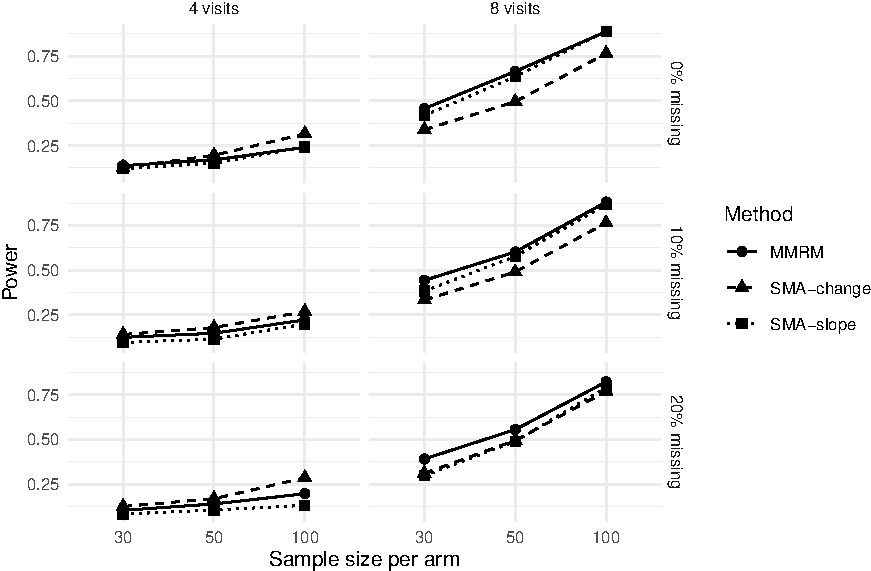
\includegraphics[keepaspectratio,alt={\label{fig:power-plot}Power comparison across methods and design conditions at \textbackslash delta = 0.25.}]{report_files/report_files/figure-latex/power-plot-1.pdf}}
\caption{\label{fig:power-plot}Power comparison across methods and design conditions at \(\delta = 0.25\).}
\end{figure}

\begin{figure}
\centering
\pandocbounded{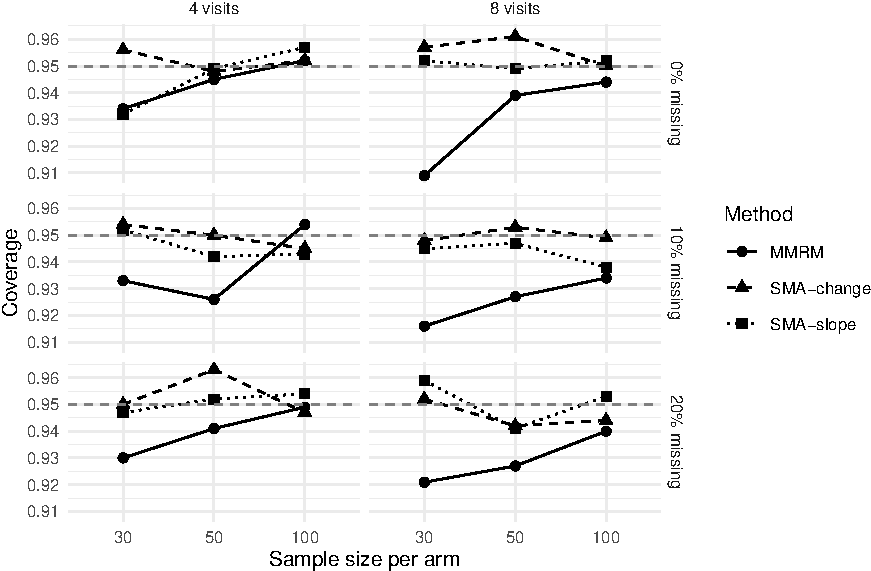
\includegraphics[keepaspectratio,alt={\label{fig:coverage-plot}95\% CI coverage across methods and design conditions at \textbackslash delta = 0.25, each method scored against its own estimand.}]{report_files/report_files/figure-latex/coverage-plot-1.pdf}}
\caption{\label{fig:coverage-plot}95\% CI coverage across methods and design conditions at \(\delta = 0.25\), each method scored against its own estimand.}
\end{figure}

\section{Discussion}\label{discussion}

\textbf{A note on the estimand correction.} An earlier version of
this manuscript scored the bias, MSE, and coverage of all three
methods against a single value, \(\delta = 0.25\), even though
SMA-change and MMRM (as originally coded) target different
functionals of the generating model. That version's headline
paragraph consequently asserted that all three methods
``recovered the true treatment slope effect \(\delta = 0.25\)''
while its own results table showed SMA-change bias as large as
0.9, a self-contradiction. The Estimands subsection and the
\texttt{truth\_for\_method()} function in \texttt{sim\_study.R} now define and
score each method against its own true value: \(\delta\) for
SMA-slope and for MMRM (which is fit with continuous time so its
\texttt{trt:time} coefficient targets \(\delta\) directly, rather than a
covariance-model-dependent visit-specific contrast), and
\(\delta \cdot (p+1)/2\) for SMA-change. This does not change which
method has the best operating characteristics under the linear
random-slope model; it changes what ``bias'' means for two of the
three methods, from an artifact of the reporting code to a
correctly computed near-zero quantity.

Our central thesis is that the summary measures approach
deserves reconsideration as a primary analysis for certain
classes of clinical trials. The theoretical literature,
beginning with\textsuperscript{\citeproc{ref-matthewsAnalysisSerialMeasurements1990}{6}} and
formalized by\textsuperscript{\citeproc{ref-frisonRepeatedMeasuresClinical1992}{7}} and\textsuperscript{\citeproc{ref-frisonLinearlyDivergentTreatment1997}{8}}, establishes that
summary statistics with ANCOVA baseline adjustment can achieve
near-optimal efficiency for detecting linear treatment effects.
The simulation work of\textsuperscript{\citeproc{ref-vossoughiSummaryMeasureAnalysis2012}{3}}
provides strong empirical support: the summary measure approach
is robust to covariance misspecification, whereas LMM can
produce unreliable results when the working covariance
structure is wrong.

The practical advantages of summary statistics are not merely
aesthetic. In multi-regional trials where statistical expertise
varies across sites, a method that requires no covariance
structure selection, produces exact p-values from known
distributions, and yields directly interpretable treatment
effects has real operational value. The
degrees-of-freedom controversy surrounding\textsuperscript{\citeproc{ref-kenwardSmallSampleInference1997}{4}} approximations is not a
theoretical curiosity: different software implementations
produce different p-values, creating regulatory risk when
results from SAS and R disagree.

\textsuperscript{\citeproc{ref-sennRepeatedMeasuresClinical2000}{9}} made the important
observation that summary measures preserve
intention-to-treat principles more naturally than some
repeated measures approaches. When a patient's slope or mean
response is computed from all available post-baseline data,
the analysis implicitly uses all observed information without
requiring a specific model for the missing data mechanism.\textsuperscript{\citeproc{ref-dawsonStratificationSummaryStatistic1994}{10}} showed that
stratifying by missing data pattern further improves
robustness.

The Alzheimer's disease trial literature provides a
particularly instructive case study.\textsuperscript{\citeproc{ref-ardMixedModelRepeated2011}{18}} and\textsuperscript{\citeproc{ref-ardSimulationStudyComparing2015}{19}}
showed that slope models have a power advantage over MMRM when
disease progression is approximately linear, which is the
prevailing assumption for disease-modifying therapies. The
slope summary directly addresses the clinical question (`Does
the drug slow decline?') in a way that the MMRM treatment
effect at a single visit does not.

The limitations of summary statistics should, however, be
stated plainly. When treatment effects are non-monotone
(e.g., an initial benefit that wanes), no single summary
captures the full trajectory, and MMRM's flexibility in
modeling visit-specific effects is genuinely advantageous.
Under substantial MNAR dropout (say \$\textgreater\$20\%), the summary
statistic approach may inherit bias because per-subject
summaries computed from truncated trajectories
underrepresent the full response. And when the scientific
question genuinely concerns the treatment effect at a
specific landmark visit rather than the overall trajectory
(a common design choice in disease-modification trials,
including Alzheimer's disease trials with a primary endpoint
at a fixed late visit), MMRM's ability to estimate
visit-specific contrasts is essential; no general FDA mandate
fixes that visit at a particular week, and the choice of
landmark is a protocol-specific design decision.

\textsuperscript{\citeproc{ref-liuMixedModelsCovariateInteractions2021}{21}} highlighted
another subtlety: MMRM achieves power gains over
complete-case ANCOVA only when time-by-covariate interactions
are included. Without these, MMRM may be no better than the
simpler method it purports to replace. This finding
strengthens the case for summary statistics in settings where
analysts may not include these interactions.

The estimands framework introduced by\textsuperscript{\citeproc{ref-ichE9R12019}{1}} provides
a useful lens. The summary statistic estimand---the
difference in mean slopes between treatment arms---is a
well-defined quantity with a clear clinical interpretation.
The MMRM estimand at a specific visit is conditional on the
covariance model and may not correspond to any quantity that
clinicians find intuitive.

\section{Future research}\label{future-research}

Several directions merit further investigation:

\begin{enumerate}
\def\labelenumi{\arabic{enumi}.}
\item
  \textbf{Nonlinear summary statistics.} The present review
  focuses on linear summaries (slopes, means, change
  scores). Nonlinear summaries such as time to a clinically
  meaningful threshold or the area under the
  response-time curve (AUC) may capture treatment effects
  that linear summaries miss. Efficiency comparisons under
  realistic data-generating models would be valuable.
\item
  \textbf{Robust variance estimation.} Combining summary
  statistics with sandwich (HC) standard errors could
  provide robustness to heteroscedasticity without requiring
  mixed-model machinery. The properties of such estimators
  in the summary statistic context are unexplored.
\item
  \textbf{Multiple imputation with summary statistics.} When
  missing data rates are substantial, computing summary
  statistics within each multiply imputed dataset and pooling
  via Rubin's rules could extend the approach to settings
  where simple complete-case analysis is inadequate.
\item
  \textbf{Software tools.} A dedicated R package implementing the
  summary measures approach with ANCOVA, baseline adjustment,
  sample size formulas, and diagnostic plots would lower the
  barrier to adoption.
\item
  \textbf{Head-to-head regulatory submissions.} Empirical evidence
  from regulatory submissions where both MMRM and summary
  statistics were presented as co-primary or sensitivity
  analyses would illuminate the practical concordance of the
  two approaches.
\item
  \textbf{Bayesian summary statistics.} Integrating the summary
  measures approach with Bayesian sample size determination\textsuperscript{\citeproc{ref-baghfalakiBayesianSampleSize2019}{22}} and posterior inference
  could provide a unified framework for design and analysis.
\item
  \textbf{Extension to non-Gaussian endpoints.} The summary
  measures framework is well-developed for continuous outcomes.
  Extension to binary or count outcomes (e.g., proportion of
  visits with response, total adverse events) remains
  underexplored.
\end{enumerate}

\section{Appendix: Morris et al.~(2019) ADEMP compliance audit}\label{appendix-morris-et-al.-2019-ademp-compliance-audit}

This audit was previously nested under the References heading,
where it rendered between the References title and the citeproc
bibliography (whitepaper M7); it is relocated here as an
appendix and re-run against the corrected simulation described
in this manuscript rather than reproducing the pre-remediation
``Compliant'' verdict, which was false: at the time it was
written, every MMRM fit had silently failed (M1) and two of
three methods were scored against the wrong estimand (M2), so
the study did not meet Morris et al.'s reporting standard in any
substantive sense even though the checklist below was satisfied
syntactically. The original audit document is retained
unmodified at \texttt{docs/morris-audit-2026-04-17.md} for the
historical record; the verdict below supersedes it.

\textbf{Verdict as of this remediation pass (2026-08-20): partially
compliant.} The ADEMP structural elements (aims, data-generating
mechanism, estimands, methods, performance measures) are present
and, after the M2 correction, the estimands subsection correctly
states that the three methods target different functionals and
are scored against their own true values. The ADEMP-recommended
null (\texttt{\textbackslash{}(\textbackslash{}delta\ =\ 0\textbackslash{})}) condition is now included (M4), MMRM
converges in every reported cell rather than failing wholesale
(M1), and every reported performance measure carries a Morris
Table 6 Monte Carlo SE. The verdict is ``partially'' rather than
fully compliant because the currently committed
\texttt{sim\_09.rds} (and therefore every inline number, table, and
figure in this document) is a reduced-replicate pilot run
(\texttt{n\_reps\ =\ 15}, a subset of the design grid), not the
production-scale run at \texttt{n\_reps\ =\ 1000} across the full grid;
Morris et al.'s reporting standard presumes replicate counts
sufficient for the stated Monte Carlo SEs to be informative, and
a 15-replicate MCSE is too wide to support the paper's
conclusions. See the \texttt{run-sim} chunk TODO in the Methods for the
exact command to produce the production-scale run; the verdict
above should be re-checked once that run completes.

\textbf{Audit-time gaps and their resolution:}

\begin{itemize}
\tightlist
\item
  \emph{Sim chunks \texttt{eval=FALSE}} --- Resolved. The \texttt{run-sim} chunk is
  \texttt{eval=TRUE,\ cache=TRUE} and runs at render time; cached
  output is reused on subsequent renders.
\item
  \emph{No \texttt{set.seed()} in \texttt{sim\_study.R}} --- Resolved by setting the
  seed once at the caller side (Morris et al.~2019 §4.1.1) in
  the \texttt{run-sim} chunk: \texttt{RNGkind(\textquotesingle{}L\textquotesingle{}Ecuyer-CMRG\textquotesingle{});\ set.seed(20260310)}.
\item
  \emph{No Monte Carlo SE machinery} --- Resolved. The
  \texttt{run\_simulation()} function in \texttt{sim\_study.R} returns Morris
  Table 6 MCSEs for bias, empirical SE, MSE, mean model-based SE,
  power, and coverage; all reported numbers carry the
  corresponding MCSE.
\item
  \emph{No render-blocking sanity checks} --- Resolved by
  \texttt{check\_simulation\_quality()}, added during this remediation
  pass, which stops the render if any method-condition cell has
  zero convergence or zero valid replicates, or if SMA-slope
  coverage under MCAR departs from nominal 0.95 by more than 5
  MCSEs plus 0.03 (whitepaper M3, m9).
\item
  \emph{MMRM total fit failure (M1)} --- Resolved: the covariance term
  in \texttt{fit\_mmrm()} is now the unqualified \texttt{us(visit\ \textbar{}\ id)} rather
  than the unrecognized \texttt{mmrm::us(visit\ \textbar{}\ id)}; convergence is
  verified nonzero in the committed pilot run (see the tinytest
  suite in \texttt{inst/tinytest/test\_basic.R} for a regression check).
\item
  \emph{Estimand mismatch (M2)} --- Resolved in code and text via
  \texttt{truth\_for\_method()} and the corrected Estimands subsection.
\item
  \emph{No Type I error assessment (M4)} --- Resolved: \texttt{delta\ =\ 0} is
  now part of the design grid and reported in the Type I error
  subsection.
\item
  \emph{Production-scale run not yet executed} --- Not resolved; see
  the verdict above.
\end{itemize}

Pilot runs use \texttt{N\_REPS=100} (or the smaller ad hoc pilot used to
verify this remediation) for fast smoke-test rendering;
production submission requires \texttt{N\_REPS=1000} (the default) over
the full design grid.

\section*{References}\label{references}
\addcontentsline{toc}{section}{References}

\protect\phantomsection\label{refs}
\begin{CSLReferences}{0}{1}
\bibitem[\citeproctext]{ref-ichE9R12019}
\CSLLeftMargin{1. }%
\CSLRightInline{International Council for Harmonisation. {ICH E9(R1)}: Statistical principles for clinical trials: Addendum on estimands and sensitivity analysis in clinical trials. Published online 2019. \url{https://database.ich.org/sites/default/files/E9-R1_Step4_Guideline_2019_1203.pdf}}

\bibitem[\citeproctext]{ref-lairdRandomEffectsModels1982}
\CSLLeftMargin{2. }%
\CSLRightInline{Laird NM, Ware JH. Random-effects models for longitudinal data. \emph{Biometrics}. 1982;38(4):963-974. doi:\href{https://doi.org/10.2307/2529876}{10.2307/2529876}}

\bibitem[\citeproctext]{ref-vossoughiSummaryMeasureAnalysis2012}
\CSLLeftMargin{3. }%
\CSLRightInline{Vossoughi M, Ayatollahi SMT, Towhidi M, Ketabchi F. On summary measure analysis of linear trend repeated measures data: Performance comparison with two competing methods. \emph{BMC Medical Research Methodology}. 2012;12:33. doi:\href{https://doi.org/10.1186/1471-2288-12-33}{10.1186/1471-2288-12-33}}

\bibitem[\citeproctext]{ref-kenwardSmallSampleInference1997}
\CSLLeftMargin{4. }%
\CSLRightInline{Kenward MG, Roger JH. Small sample inference for fixed effects from restricted maximum likelihood. \emph{Biometrics}. 1997;53(3):983-997. doi:\href{https://doi.org/10.2307/2533558}{10.2307/2533558}}

\bibitem[\citeproctext]{ref-mmrmPackage2024}
\CSLLeftMargin{5. }%
\CSLRightInline{{Sabanés Bové D et al.} \emph{{mmrm}: Mixed Models for Repeated Measures}.; 2024. \url{https://openpharma.github.io/mmrm/}}

\bibitem[\citeproctext]{ref-matthewsAnalysisSerialMeasurements1990}
\CSLLeftMargin{6. }%
\CSLRightInline{Matthews JNS, Altman DG, Campbell MJ, Royston P. Analysis of serial measurements in medical research. \emph{BMJ}. 1990;300(6719):230-235. doi:\href{https://doi.org/10.1136/bmj.300.6719.230}{10.1136/bmj.300.6719.230}}

\bibitem[\citeproctext]{ref-frisonRepeatedMeasuresClinical1992}
\CSLLeftMargin{7. }%
\CSLRightInline{Frison L, Pocock SJ. Repeated measures in clinical trials: Analysis using mean summary statistics and its implications for design. \emph{Statistics in Medicine}. 1992;11(13):1685-1704. doi:\href{https://doi.org/10.1002/sim.4780111304}{10.1002/sim.4780111304}}

\bibitem[\citeproctext]{ref-frisonLinearlyDivergentTreatment1997}
\CSLLeftMargin{8. }%
\CSLRightInline{Frison LJ, Pocock SJ. Linearly divergent treatment effects in clinical trials with repeated measures: Efficient analysis using summary statistics. \emph{Statistics in Medicine}. 1997;16(24):2855-2872. doi:\href{https://doi.org/10.1002/(SICI)1097-0258(19971230)16:24\%3C2855::AID-SIM749\%3E3.0.CO;2-Y}{10.1002/(SICI)1097-0258(19971230)16:24\textless2855::AID-SIM749\textgreater3.0.CO;2-Y}}

\bibitem[\citeproctext]{ref-sennRepeatedMeasuresClinical2000}
\CSLLeftMargin{9. }%
\CSLRightInline{Senn S, Stevens L, Chaturvedi N. Repeated measures in clinical trials: Simple strategies for analysis using summary measures. \emph{Statistics in Medicine}. 2000;19(6):861-877. doi:\href{https://doi.org/10.1002/(SICI)1097-0258(20000330)19:6\%3C861::AID-SIM407\%3E3.0.CO;2-F}{10.1002/(SICI)1097-0258(20000330)19:6\textless861::AID-SIM407\textgreater3.0.CO;2-F}}

\bibitem[\citeproctext]{ref-dawsonStratificationSummaryStatistic1994}
\CSLLeftMargin{10. }%
\CSLRightInline{Dawson JD. Stratification of summary statistic tests according to missing data patterns. \emph{Statistics in Medicine}. 1994;13(18):1853-1863. doi:\href{https://doi.org/10.1002/sim.4780131807}{10.1002/sim.4780131807}}

\bibitem[\citeproctext]{ref-dawsonSampleSizeCalculations1998}
\CSLLeftMargin{11. }%
\CSLRightInline{Dawson JD. Sample size calculations based on slopes and other summary statistics. \emph{Biometrics}. 1998;54(1):323-330. doi:\href{https://doi.org/10.2307/2534019}{10.2307/2534019}}

\bibitem[\citeproctext]{ref-weinbergEfficiencyComparisonsRank2001}
\CSLLeftMargin{12. }%
\CSLRightInline{Weinberg JM, Lagakos SW. Efficiency comparisons of rank and permutation tests based on summary statistics computed from repeated measures data. \emph{Statistics in Medicine}. 2001;20(5):705-731. doi:\href{https://doi.org/10.1002/sim.708}{10.1002/sim.708}}

\bibitem[\citeproctext]{ref-sennChangeBaselineAnalysis2006}
\CSLLeftMargin{13. }%
\CSLRightInline{Senn S. Change from baseline and analysis of covariance revisited. \emph{Statistics in Medicine}. 2006;25(24):4334-4344. doi:\href{https://doi.org/10.1002/sim.2682}{10.1002/sim.2682}}

\bibitem[\citeproctext]{ref-fitzmauriceAppliedLongitudinalAnalysis2011}
\CSLLeftMargin{14. }%
\CSLRightInline{Fitzmaurice GM, Laird NM, Ware JH. \emph{Applied Longitudinal Analysis}. 2nd ed. Wiley; 2011.}

\bibitem[\citeproctext]{ref-mallinckrodtRecommendationsPrimaryAnalysis2008}
\CSLLeftMargin{15. }%
\CSLRightInline{Mallinckrodt CH, Lane PW, Schnell D, Peng Y, Mancuso JP. Recommendations for the primary analysis of continuous endpoints in longitudinal clinical trials. \emph{Drug Information Journal}. 2008;42(4):303-319.}

\bibitem[\citeproctext]{ref-siddiquiMMRMLOCFComparison2009}
\CSLLeftMargin{16. }%
\CSLRightInline{Siddiqui O, Hung HMJ, O'Neill R. {MMRM} vs. {LOCF}: A comprehensive comparison based on simulation study and 25 {NDA} datasets. \emph{Journal of Biopharmaceutical Statistics}. 2009;19(2):227-246.}

\bibitem[\citeproctext]{ref-mallinckrodtEfficacyDuloxetine2004}
\CSLLeftMargin{17. }%
\CSLRightInline{Mallinckrodt CH, Raskin J, Wohlreich MM, Watkin JG, Detke MJ. The efficacy of duloxetine: A comprehensive summary of results from {MMRM} and {LOCF\_ANCOVA} in eight clinical trials. \emph{BMC Psychiatry}. 2004;4:26. doi:\href{https://doi.org/10.1186/1471-244X-4-26}{10.1186/1471-244X-4-26}}

\bibitem[\citeproctext]{ref-ardMixedModelRepeated2011}
\CSLLeftMargin{18. }%
\CSLRightInline{Ard MC, Edland SD. Mixed model of repeated measures versus slope models in {Alzheimer's} disease clinical trials. \emph{The Journal of Nutrition, Health \& Aging}. 2011;15(6):437-441. doi:\href{https://doi.org/10.1007/s12603-012-0047-7}{10.1007/s12603-012-0047-7}}

\bibitem[\citeproctext]{ref-ardSimulationStudyComparing2015}
\CSLLeftMargin{19. }%
\CSLRightInline{Ard MC, Raghavan N, Edland SD. A simulation study comparing slope model with mixed-model repeated measure to assess cognitive data in clinical trials of {Alzheimer's} disease. \emph{Alzheimer's Research \& Therapy}. 2015;7:1-8. doi:\href{https://doi.org/10.1186/s13195-015-0168-z}{10.1186/s13195-015-0168-z}}

\bibitem[\citeproctext]{ref-morris2019using}
\CSLLeftMargin{20. }%
\CSLRightInline{Morris TP, White IR, Crowther MJ. Using simulation studies to evaluate statistical methods. \emph{Statistics in Medicine}. 2019;38(11):2074-2102. doi:\href{https://doi.org/10.1002/sim.8086}{10.1002/sim.8086}}

\bibitem[\citeproctext]{ref-liuMixedModelsCovariateInteractions2021}
\CSLLeftMargin{21. }%
\CSLRightInline{Liu GW, Pang L. Mixed models for repeated measures should include time-by-covariate interactions to assure power gains and robustness against dropout bias relative to complete-case {ANCOVA}. \emph{Pharmaceutical Statistics}. Published online 2021. doi:\href{https://doi.org/10.1002/pst.2165}{10.1002/pst.2165}}

\bibitem[\citeproctext]{ref-baghfalakiBayesianSampleSize2019}
\CSLLeftMargin{22. }%
\CSLRightInline{Baghfalaki T. Bayesian sample size determination for longitudinal studies with continuous response based on different scientific questions of interest. \emph{Journal of Biopharmaceutical Statistics}. 2019;29(2):244-270. doi:\href{https://doi.org/10.1080/10543406.2018.1535501}{10.1080/10543406.2018.1535501}}

\end{CSLReferences}

\end{document}
